\chapter{线性代数拾遗}\label{appx:LA}

\section{线性空间}

带有满足结合律的二元运算的非空集称\textbf{半群}(semigroup)。存在单位元的半群称\textbf{幺半群}(monoid)。元素皆可逆的幺半群正是群。
\textbf{同态}(homomorphisms)是保持群结构的映射 $f \in \hom(G_1, G_2 ) \Leftrightarrow f (g_1 h_1 )=f (g_1 ) f (h_1 )$。
单位元和逆元是唯一的,因为假设 $\bar 1',\bar 1$ 是单位元,则 $\bar 1'=\bar 1'\bar 1=\bar 1$;假设 $z,\bar x$ 是 $x$ 的负元,则 $z=z\bar 1=z(x\bar x)=(zx)\bar x=\bar 1\bar x=\bar x$。

\textbf{环}(ring)具有两种分别称为加法和乘法的运算,其中加法应构成交换群(Abel 群),乘法应满足结合律,并同加法一起满足分配律。加法单位元称为\textbf{零元},加法逆元称为\textbf{负元}。不混淆时零元记作 $0$,而 $x$ 的负元记作 $-x$。
若乘法满足交换律,则称\textbf{交换环}或 \textbf{Abel 环}。存在乘法单位元的环称\textbf{幺环}。非零元在乘法上可逆的环称\textbf{除环}。交换幺除环称为\textbf{域}(field),常记作空心字符,如 $\mathbb{K}$。称域对其加法、乘法是\textbf{封闭的}。由于零元不可逆,故通常要求域首先至少有零元和乘法单位元。
环 $R$ 的一个\textbf{双边理想}(2-sided ideal) $I$ 是 $R$ 的一个子环,且满足 
\[r \in R, a \in I \To r a \in I, a r \in I.\]
可用显然的方式定义\textbf{左理想}和\textbf{右理想}。

群、环、域都只考虑某个集合的\textbf{内部运算}。我们当然也能考虑另一集合来构造所谓的\textbf{外部运算}。通常我们会在群上,加上一个由环给出的外部运算,这就是某环上的\textbf{模}(module)。
给定环 $R$,\textbf{左 $R$-模} $X$ 是一个交换群,且带有另一称为外部乘法的运算 $R \times X \rightarrow X$,满足对 $\forall \alpha,\beta \in R, x,y \in X$ 有如下分配律和结合律:
\[(\alpha+\beta) x=\alpha x+\beta x,\quad \alpha(x+y)=\alpha x+\alpha y,\quad (\alpha\beta)x=\alpha(\beta x).\]
若 $R$ 是幺环,则还要求其乘法单位元 $1$ 使 $1x=x$。\textbf{右 $R$-模}的定义是显然的。

\textbf{代数}(algebra)首先是幺环 $R$ 上的模 $X$,且要给定另一称为乘积的内部运算,使得 $X$ 自身是环,并对 $\forall \alpha \in R, x,y \in X$ 有 $\alpha(xy)=(\alpha x) y=x(\alpha y)$。可见代数上有五种运算:$R$ 的加法和乘法、$X$ 的加法和乘积、外部乘法。

进而回顾一下,域 $\mathbb F$ 上的\textbf{线性空间}其实就是 $\mathbb F$-模。由于 $\mathbb F$ 是域,选取左模或右模其实无关宏旨。一般取实数域 $\R$ 或复数域 $\C$,相应有实线性空间和复线性空间。显然 $\mathbb F$ 自身可以成为 $\mathbb F$-线性空间。线性空间的元素称为\textbf{向量}或\textbf{矢量}。其中内部运算称为(逐点)加法,外部运算称为数乘。物理上常称为\textbf{线性叠加原理},而将矢量画成笔直的箭头。可以看到,$V$ 在赋予某种乘法后是一个代数,可称\textbf{线性代数},比如内积空间或者张量积空间。当然,线性代数在现在更多指此概念所发展的一套学说。

设线性空间 $V$。某非空 $S\subset V$ 内元素的全体线性组合构成子空间 $\operatorname{span}B$,称为由 $B$ 张成的。若存在线性无关的非空子集 $B$ 使 $\operatorname{span}B=V$,则称 $B$ 是 $V$ 的一个\textbf{基}(basis)或一组\textbf{基矢}(basis vectors)。若 $B$ 是有限集,则称 $V$ 是\textbf{有限维的},可定义维数 $\dim V:=|B|$。易知任意基的元素个数一致,由此维数是良定义的。若 $B$ 是无限集,也即任意有限矢量组 $\{e_\mu\}_{\mu=1}^n$ 都不构成基,则称 $V$ 是\textbf{无限维的}。典型例子是 $[a, b] \subset \R$ 上连续复函数构成无限维复线性空间 $C[a, b]$,直观上是因为 $[a, b]$ 有无穷多自由度,从而总存在函数不能有限表出。
映射 $A:V\to V$ 称为 $V$ 上的\textbf{算子}、\textbf{算符}(operator)或\textbf{变换}。
有限维里有很多结论不能简单推广至无限维,否定这些结论带来了更多“反直觉”的性质。相对论的物理量主要属于有限维。

\begin{definition}
    \textbf{泛函}严格指无限维 $V$ 上的函数。
\end{definition}

\begin{remark}
    曾用拉氏理论理解泛函,而 Fréchet 空间的确是无限维线性空间。
\end{remark}

易知 $x\in V$ 可由任意基 $\{e_\mu\}$ 唯一地线性表示,称系数组 $\{k^\mu\}$ 为 $x$ 由 $\{e_\mu\}$ 表出的\textbf{分量},有限维时写作 $(k^1,\cdots,k^n)^\mathrm{T}$。欲谈及同一矢量在不同基间的分量变换,先要给定基变换。
设 $\{e_\mu\},\{e'_\mu\}$ 是线性空间 $V$ 上两组不同的基,某矢量 $v\in V$ 在两组基下的分量分别是 $\{v^\mu\},\{v'^\mu\}$。设基矢 $e_\mu^{\prime}$ 在 $\{e_\mu\}$ 下的展开为
\eq{
e'_\mu=A^\nu{ }_\mu e_\nu,
}
其中 $A$ 也叫过渡矩阵。两个基皆线性无关,故过渡矩阵可逆。于是由 $v'^\mu e'_\mu=v^\nu e_\nu$ 得 $v'^\mu A^\nu{ }_\mu e_\nu=v^\nu e_\nu$,由基的线性无关性知 $v'^\mu A^\nu{ }_\mu =v^\nu$,故
\eq{
    v'^\mu=(A^{-1})^\mu{}_\nu v^\nu.
}
因此基变换和分量变换是互逆的。

\section{对偶空间}

以 $\mathbb F$-线性空间为对象、线性映射为态射,构建\textbf{线性空间范畴} $\cate{Vect}(\mathbb F)$。

置 $f\in\hom(V,W)$。线性变换或线性算子即取 $W=V$ 的 $f\in\operatorname{End} V$。$W=\mathbb F$ 时称为线性函数。设 $V$ 的一个基 $\{e_\mu\}$,对 $V$ 中任意矢量 $k^\mu e_\mu$ 有 $f(k^\mu e_\mu)=k^\mu f(e_\mu)$。故其实只要知道 $\{e_\mu\}$ 在 $f$ 下的像组 $\{f(e_\mu)\}$,则 $V$ 中任意矢量在 $f$ 下的像就确定了,即线性映射完全由基的作用效果确定。显然 $A\in\hom(U,V),B\in\hom(V,W)$ 的复合也线性,即 $BA\in\hom(U,W)$。

假若 $f$ 还是双射,则 $f\in\mathrm{Isom}(V, W)$ 且 $f^{-1}\in\hom(W,V)$。换言之,$V,W$ 的线性双射为同构。若存在同构,则称 $V,W$ 互为\textbf{线性同构的},记作 $U\cong V$。有限维时易证等价于 $\dim U=\dim V$。易知 $f$ 是单射时,核为 $\ker f:=\{\alpha\in V:f(\alpha)=0\}=\{0\}$;$f$ 是满射时像为 $\Im f=W$。秩为 $\rank f:=\dim \Im f$,可证满足 $\dim \ker f + \dim \Im f = \dim V$。故若 $f$ 单射,则 $\Im f\cong V$。对线性变换而言,这说明单射等价于满射。换言之,满秩线性变换乃 $V$ 自同构。

对任意线性空间 $V,W$,只要对 $\hom(V,W)$ 定义如下加法、数乘、零元:$\forall f,g\in \hom(V,W),v\in V,\alpha\in\mathbb F$ 有
\[(f+g)(v):=f(v)+g(v),\quad (\alpha f)(v):=\alpha f(v),\quad 0(v):=0,\]
则 $\hom(V,W)$ 成为了线性空间。一般考虑线性函数。任意线性函数 $\omega\in V^*:=\hom(V,\mathbb F)$ 称为\textbf{对偶矢量},称 $V^*$ 为\textbf{对偶空间}。
比如,行向量空间就是列向量空间的对偶空间。
考虑从原来的 $V$ 来产生 $V^*$ 的基。方法是,假设 $\{e_\mu\}$ 是 $V$ 的一个基,则定义 $V^*$ 中有一组元素 $\{e^\mu\}$ 满足
\eq{ e^\mu(e_\nu):=\delta^\mu_\nu,}
进而由线性性可导出它对 $V$ 任意元素的作用情况,即 $e^\mu(A)=A^\mu$。再证明 $\{e^\mu\}$ 确实是一个基:对任意 $\omega\in V^*$ 设
\eq{
    \omega_\mu:=\omega(e_\mu),
}
则必能展开成 $\omega=\omega_\mu e^\mu$,因为两边作用于任意 $V$ 中元素即可,如 $\omega(e_\nu)=\omega_\mu e^\mu(e_\nu)=\omega_\nu$;显然线性无关:$0=\omega_\mu e^\mu(e_\nu)=\omega_\nu$。这说明 $\dim V^*=\dim V$ 或者 $V\cong V^*$。按此关系给出的 $\{e^\mu\}$ 就称 $\{e_\mu\}$ 的\textbf{对偶基}。

$V,V^*$ 间的同构当然是不唯一的。注意到 $\{e_\mu\}$ 到其对偶基 $\{e^\mu\}$ 的线性映射就是同构,那这会随着 $\{e_\mu\}$ 的不同选取而产生不同的同构。
若要有充分理由挑选出特殊同构,需另加结构限制之。
比如度规就建立了 $V,V^*$ 的特殊同构。

对偶操作不必继续“套娃”。设 $V^{**}=\hom(V^*,\mathbb F)$,下面说明可给 $V,V^{**}$ 找到同构,它不依赖于基的人为选取。用基底展开后有 $\omega(A)=\omega_\mu A^\mu=A^\mu\omega_\mu$,说明如果认为映射可交换,矢量也可成为对偶矢量的线性函数,只需定义 $i_V:V\to V^{**}$ 使得 $i_V A$ 满足 $i_V A(\omega):=\omega(A)$,
有时 $i_V A$ 简记作 $A^{**}$。显然 $i_V\in\mathrm{Isom}(V,V^{**})$。定义 $f\in\hom(V,W)$ 的对偶 $f^*\in\hom(W^*, V^*)$ 使得 $\forall\lambda\in W^*,A\in V$ 有
\eq{
    (f^*(\lambda))(A)=\lambda(f(A)).
}
显然恒等变换 $\mathrm{id}_V\in \operatorname{Aut} V$ 的对偶为 $\mathrm{id}_V^*=\mathrm{id}_{V^*}$;复合映射满足 $(f\circ g)^*=g^*\circ f^*$。进而取逆映射进行复合可知,若 $f$ 是同构则 $f^*$ 也是。
可证对任意线性 $f$,此同构是自然的:
\[\begin{tikzcd}
    V \arrow[r, "i_V"] \ar[d, "f"'] & V^{**} \arrow[d, "f^{**}"] \\
    W \arrow[r, "i_W"] & W^{**} ,
\end{tikzcd}\]
故被称为\textbf{自然同构}。$f$ 取决于对基的作用效果,故换言之,自然同构不依赖于基。实践中经常把自然同构直接写成等号,即 $V=V^{* *}$。将二者做认同后,省略同构符号可写成 $\omega(A)=A(\omega)$,数学上常写成 $\langle\omega,A\rangle$,这说明对偶矢量与矢量之间有天生的(god-given)乘法。且可证,不存在 $i_V\in\mathrm{Isom}(V,V^*)$ 使下图对任意线性 $f$ 交换:
\[\begin{tikzcd}
    V \arrow[r, "i_V"] \ar[d, "f"'] & V^{*} \\
    W \arrow[r, "i_W"] & W^{*} \arrow[u, "f^{*}"'],
\end{tikzcd}\]
故只有 $V,V^{* *}$ 间才能有自然同构。读者只需取以 $\R$ 为线性空间的特例就可证明。真正有用的是 $V,V^*$,好似两面镜子相互反射。设 $v=v^\mu e_\mu$,自然有 $v^\mu=v^\nu \langle e^\mu,e_\nu\rangle=v(e^\mu)$。
最后来研究各种分量、基变换的关系。
\begin{theorem}
    若 $V$ 中有一基变换 $e_\mu^{\prime}=A^\nu{ }_\mu e_\nu$,则相应的对偶基变换为
\eq{
e^{\prime \mu}=(A^{-\mathrm{T}})_\nu{ }^\mu e^{\nu}=(A^{-1})^\mu{ }_\nu e^{\nu}.
}
这说明对偶矢量 $\omega=\omega_\mu e^\mu$ 的坐标变换为 $\omega_\mu'=A^\nu{}_\mu\omega_\nu$。
\end{theorem}

\begin{proof}
    只需等式两边作用于 $e_\alpha^{\prime}$:
    \begin{align*}({A}^{-\mathrm{T}})_\nu{}^\mu\langle e^{\nu}, e_\alpha^{\prime}\rangle & =(A^{-\mathrm{T}})_\nu{ }^\mu A^\beta{}_\alpha\langle e^{\nu}, e_\beta\rangle  =(A^\mathrm{T})_\alpha{ }^\beta (A^{-\mathrm{T}})_\nu{ }^\mu \delta_\beta^\nu\\ &=(A^\mathrm{T})_\alpha{ }^\nu (A^{-\mathrm{T}})_\nu{ }^\mu=\delta_\alpha^\mu=\langle e^{\prime \mu}, e_\alpha^{\prime}\rangle,\end{align*}
    遂见结果相同。
\end{proof}

% 协变逆变的交换图

与矢量基相同形式变换的称为协变,与矢量基相反形式变换的称为逆变。

% 这种变换形式称为逆变,新量$=$矩阵$\times$旧量。原基底满足 $e_\nu={(A^{-1})}^\mu{}_\nu e^\prime_\mu$,称为协变,旧量$=$矩阵$\times$新量。

\section{张量空间}

\begin{definition}
    设 $\mathbb F$-线性空间 $\{X_i\}_{i=1}^k,W$。若
    $T:X_1\times\cdots\times X_k\to W$
    对任何 $X_i$ 都线性,则称\textbf{多重线性映射}。常取如下情形:
    \eq{
        T:\underbrace{V^*\times\cdots\times V^*}_{k\in\N}\times\underbrace{V\times\cdots\times V}_{l\in\N}\to \mathbb F,
    }
    称为 $V$ 上的一个\textbf{多重线性函数}或\textbf{张量}。如上即 $(k,l)$-张量,构成张量空间
\eq{
    \hom(\underbrace{V^*\times\cdots\times V^*}_{k\in\N}\times\underbrace{V\times\cdots\times V}_{l\in\N},\mathbb F)=:V^k_l.
}
\end{definition}
\begin{remark}
    用分号区分上下槽,如 $T(\oo;\oo,\oo)\in V^1_2$ 可输入 $\omega,v_1,v_2$ 得 $T(\omega;v_1,v_2)\in\mathbb F$。$T$ 视为全部槽为空时的简写。
\end{remark}

\begin{figure}[ht]
    \centering
    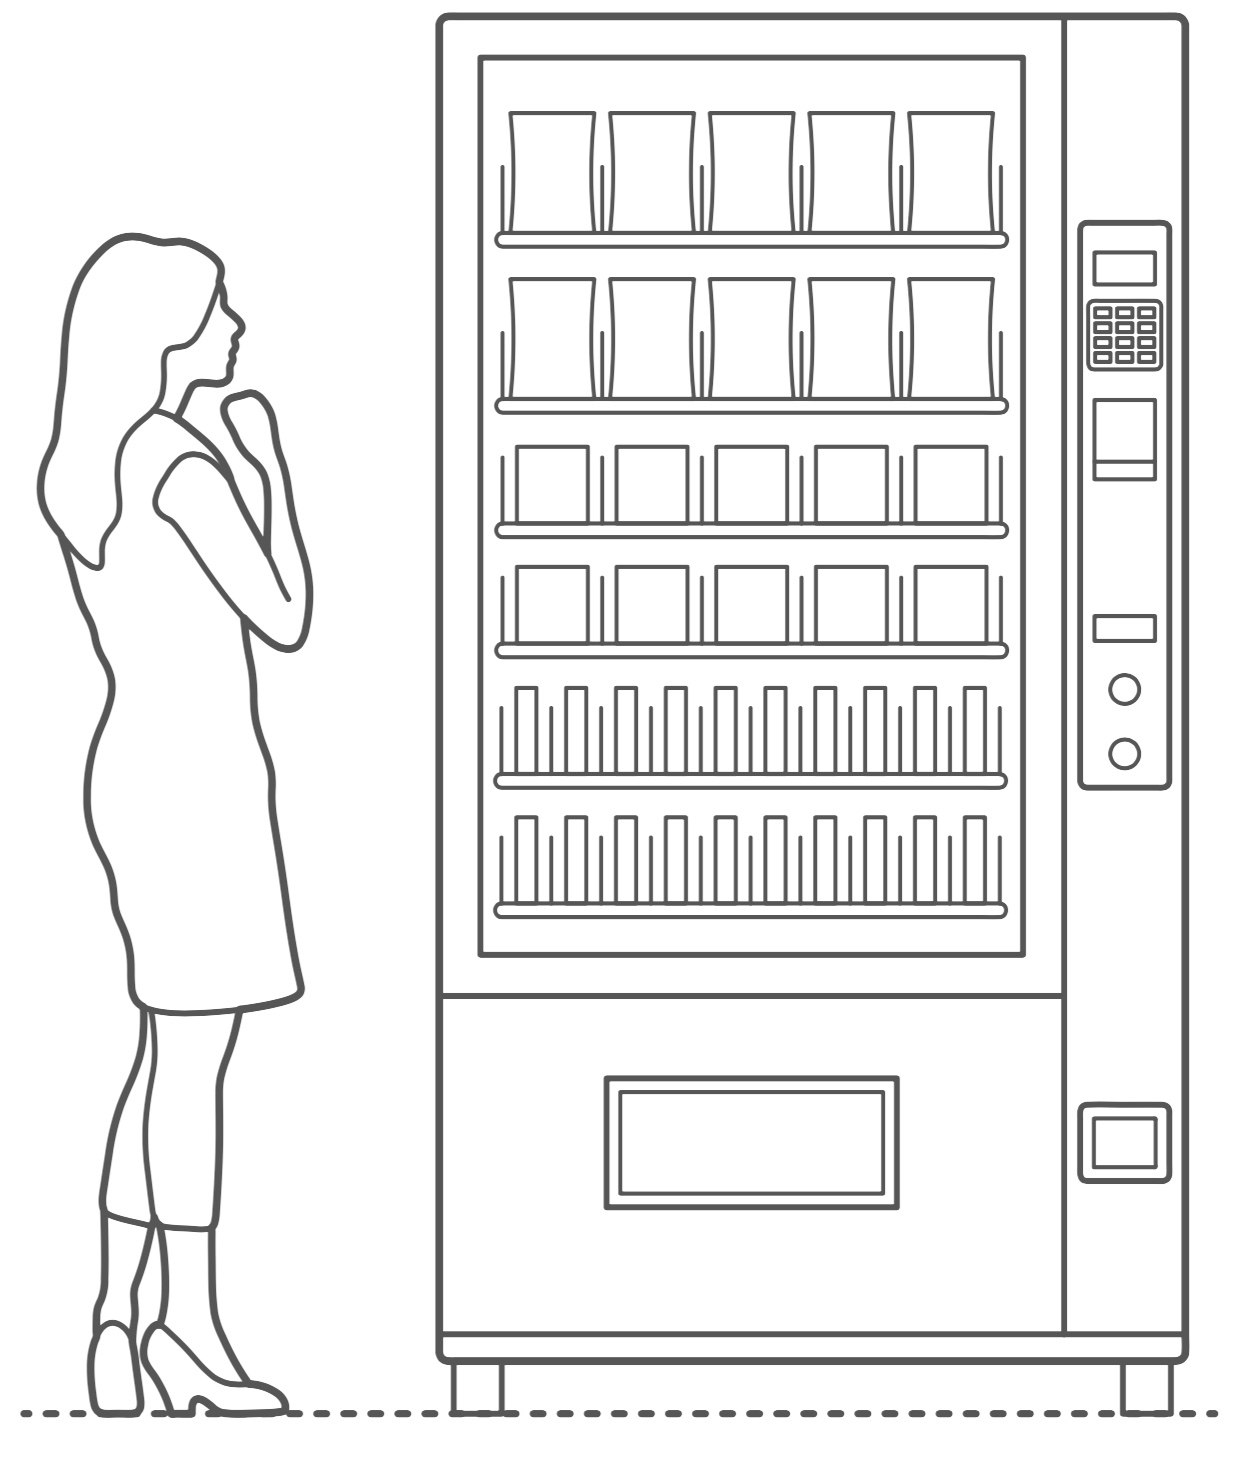
\includegraphics[width=0.4\textwidth]{fig/appx/vending.jpg}
    \caption{售货机}
    \label{fig:vending}
\end{figure}

张量与有限个矢量、对偶矢量线性地缩并出标量,因此可用多重线性函数表述。换言之,可直接称多重线性函数为张量,该定义多数情况与等价类 $[T^{\cdots}{}_{\cdots}]$ 表述等价。至少本节谈到张量均指多重线性函数。张量相比矢量、对偶矢量,无非是多出若干输入端口。
可类比从单元函数拓展到多元函数。如图 \ref{fig:vending},设想度规 $g$ 是一台具有两个槽(slat)的售货机,往槽中投入足够数量的一元纸币可获得一件商品,比如一听可乐。设某件商品需要两元纸币,则投入过程中,显示屏会不断改变数值以提示用户待支付的剩余金额,直至最终获得商品。这个过程类似于:
\[
    g(\oo,\oo)\To g(A,\oo)\in V^*\To g(A,B)\in\R.  
\]
关键在于,第一步输出的 $g(A,\oo)$ 将和之后输入的矢量 $B$ 线性地作用,最终输出实数,故相当于 $g(A,\oo)\in V^*$。类似地也有 $g(\oo,B)\in V^*$。
多重线性函数还可混合地输入矢量、对偶矢量,就好比售货机可以混合地投入硬币和纸币,只是对应的槽不同。
比如,$V$ 上的线性变换就是输入矢量且输出矢量,即 $X^\mu=T^\mu{}_\nu Y^\nu$,而矢量是对偶矢量的函数,因此线性变换又可看成矢量和对偶矢量的双线性函数,即 $(1,1)$-张量 $T^\mu{}_\nu$。比如 $\mathrm{id}_V$ 给出 $\delta^i_j A^j=A^i$,而 $\delta^i_j$ 单独看有上下槽。物理上有一例:应力张量涉及某个面上的压力,因此必定要先给定一个面法矢,这样就产生对应的一个作用力。

我们已熟知张量的线性组合、张量积、缩并,下面用映射语言重审之。

\begin{definition}  
取显然的加法、数乘、零元定义可使 $V^k_l$ 成为线性空间。这些运算即同型张量的线性组合,如 $T+ S+S+0=T+2S$。
\end{definition}

\begin{definition}
    $(k,l),(k',l')$ 型张量 $T,T'$ 的\textbf{张量积} $T\otimes T'$ 是一个 $(k+k',l+l')$-张量,使得
\begin{align}
    &T\otimes T'(\omega^1,\cdots,\omega^k,\omega^{k+1},\cdots,\omega^{k+k'};v_1,\cdots,v_l,v_{l+1},\cdots,v_{l+l'})\nonumber\\
    :=\ &T(\omega^1,\cdots,\omega^k;v_1,\cdots,v_l)\,T'(\omega^{k+1},\cdots,\omega^{k+k'};v_{l+1},\cdots,v_{l+l'}).
\end{align}
\end{definition}
\begin{remark}
    张量积有结合律,但一般不满足交换律。
\end{remark}
由于 $V^k_l$ 是线性空间,而 $V$ 有限维且 $k,l\in\N$,可讨论其维数:
\begin{theorem}
    $\dim V^k_l=(\dim V)^{k+l}.$
\end{theorem}
\begin{proof}
    设 $\{e_\mu\}$。可预料张量总能展为
    \eq{
        T={T^{\mu_1\cdots\mu_k}}_{\sigma_1\cdots\sigma_l}e_{\mu_1}\otimes\cdots\otimes e_{\mu_k}\otimes e^{\sigma_1}\otimes\cdots\otimes e^{\sigma_l},
        }
其中分量为
\eq{{T^{\mu_1\cdots\mu_k}}_{\sigma_1\cdots\sigma_l}:=T(e^{\mu_1},\cdots,e^{\mu_k};e_{\sigma_1},\cdots,e_{\sigma_l}),}
因为基底作用于相应基失的结果为
    \[e_{\mu_1}\otimes\cdots\otimes e_{\mu_k}\otimes e^{\sigma_1}\otimes\cdots\otimes e^{\sigma_l}(e^{\mu'_1},\cdots,e^{\mu'_k};e_{\sigma'_1},\cdots,e_{\sigma'_l})=\delta^{\mu'_1}_{\mu_1}\cdots\delta^{\mu'_k}_{\mu_k}\delta^{\sigma_1}_{\sigma'_1}\cdots\delta^{\sigma_l}_{\sigma'_l}.\]
基底显然线性无关。进而 $V_l^k=\mathrm{span}\{e_{\mu_1}\otimes\cdots\otimes e_{\mu_k}\otimes e^{\sigma_1}\otimes\cdots\otimes e^{\sigma_l}\}$。故 $\dim V_l^k=\prod_{i=1}^k\dim V^*\prod_{j=1}^l\dim V=(\dim V)^{k+l}$。
\end{proof}

张量空间实际上被视为\textit{线性空间张量积}的结果,即定义
    \eq{V^k_l=:\underbrace{V^*\otimes\cdots\otimes V^*}_{k\in\N}\otimes\underbrace{V\otimes\cdots\otimes V}_{l\in\N}.}
一般地,可定义不同线性空间的张量积为多重线性映射的 hom-集。换言之,矢量张量积是双线性映射 $\otimes:X\times Y\to W$,使得对任意线性空间 $Z$ 和双线性映射 $f: X\times Y\to Z$,都 $\exists!g\in\hom(W,Z)$ 满足 $f=g\circ\otimes$,即下图交换:
    \[ \begin{tikzcd}[row sep=small]
        X \times Y \arrow[rd, "f"'] \arrow[r] & X\otimes Y \arrow[d, "\exists!"] \\
        & Z.
    \end{tikzcd} \]
这称为张量积的\textbf{泛性质}。换言之,矢量张量积将 $X,Y$ 卡氏积变为其(线性空间)张量积。根据模论的相关定理,可证明 $X\otimes Y$ 一定存在,且同构意义下唯一。线性空间张量积可还原回张量及其张量积,故也是许多数学教材采用的等价定义。

\begin{theorem}
    设基变换 $e_\mu^{\prime}=A^\nu{ }_\mu e_\nu$,张量分量的变换律显然为
    \eq{
    T'^{\mu_1\cdots\mu_k}{}_{\nu_1\cdots\nu_l}=T^{\rho_1\cdots\rho_k}{}_{\sigma_1\cdots\sigma_l} (A^{-1})^{\mu_1}{ }_{\rho_1} \cdots(A^{-1})^{\mu_k}{ }_{\rho_k} A^{\sigma_1}{}_{\nu_1}   \cdots A^{\sigma_l}{}_{\nu_l}.
}
\end{theorem}
\begin{eg}
    线性变换 $T$ 的分量变换为 $T'^\mu{}_\nu= (A^{-1})^\mu{}_\rho T^\rho{}_\sigma A^\sigma{}_\nu$,即分量矩阵相似。双线性函数的分量变换为 $f'_{\mu\nu}=(A^\mathrm{T})_\mu{}^\rho f_{\rho\sigma} A^\sigma{}_\nu$,即分量矩阵合同。
\end{eg}

\begin{definition}
    $(k,l)$-张量 $ T $ 的第 $i$ 上标 $(i \leqslant k)$ 与第 $j$ 下标 $(j \leqslant l)$ 的\textbf{缩并}为
\eq{\c_{j}^{i} T:=T \big(\cdots,\hl{red}{e^{h}},\cdots ; \cdots,\hl[b]{blue}{e_{h}},\cdots\big),}
\hn{-2}{-1}{red}{第 $i$ 上槽}
\hn[b]{-2}{1}{blue}{第 $j$ 下槽}
\vspace{-0.1\baselineskip}

\noindent 其中对 $h$ 使用求和约定。缩并结果为 $(k-1,l-1)$-张量,且显然与基选择无关。
\end{definition}

缩并其实是求迹的映射版本,因此数学家会混记为 $\tr$。如线性变换 $T$ 在任意基底下矩阵的迹 $\tr T$ 就是 $(1,1)$-张量缩并,是基不变的标量。但两种符号的逻辑稍许不同:$\tr$ 是写出缩并后张量类型,$\c$ 是指明所缩指标位置。假设 $T$ 是 $(1,3)$-张量,定义 $S:=\c^1_{2}T$,分量写法是 $S_{ij}=C^{k}{}_{ikj}$,但数学上记作 $S=\tr^0_2 T$。并且 $\tr$ 的用法有时并不唯一,比如 $S_{ij}$ 求迹必须借助升指标得 $g^{ij}S_{ij}$,数学上写作 $\tr_{g}S$。
将分量语言改写为映射语言时,只需注意“先张量积再缩并”可产生各种类型的新张量。可从映射语言直接看出,其结果相当于张量对矢量、对偶矢量的作用。比如,置 $T \in V^k_l,v \in V$,则
\begin{align*}
    \c_{\cdots}^{k+1}(T \otimes v)&=T \otimes v(\cdots,e^{\mu} ; \cdots,e_{\mu},\cdots)=T(\cdots;\cdots,e_{\mu},\cdots)v(e^\mu)\\
    &=T(\cdots;\cdots,v(e^\mu)e_{\mu},\cdots)=T(\cdots;\cdots,v,\cdots);
\end{align*}
同理 $T$ 对 $\omega\in V^*$ 作用其实即 $\c_{l+1}^{\cdots}(T \otimes \omega)$。
换言之,作用就是先积后并。

\begin{definition}
    张量 $T$ 关于某两下槽\textbf{对称},若 $\forall v,w\in V$ 有
    \[
    T(\cdots,v,\cdots,w,\cdots)=T(\cdots,w,\cdots,v,\cdots).
    \]
    \textbf{反称}即
    \[
    T(\cdots,v,\cdots,w,\cdots)=-T(\cdots,w,\cdots,v,\cdots).
    \]
    上槽同理。称多个槽对称或反称,若其中任意两槽对称或反称。若对所有上/下槽,则为\textbf{全对称}、\textbf{全反称}。显然张量的对称性和其分量的对称性一致,且无关基,故可视为等价定义。

    $T\in V^0_k$ 的对称、反称部分为
\eq{
\S T:=\frac{1}{k!}\sum_{\sigma\in S_k} \sigma T, \quad\A T:=\frac{1}{k!}\sum_{\sigma\in S_k} \sgn\sigma\,\sigma T,
}
其中 $\sigma T(e_{\mu_1},\cdots,e_{\mu_k})=T(e_{\mu_{\sigma(1)}},\cdots,e_{\mu_{\sigma(k)}})=T_{\mu_{\sigma(1)}\cdots\mu_{\sigma(k)}}$ 是 $T$ 按某一 $\sigma$ 给定的一个分量。其它情形同理。
\end{definition}

\begin{theorem}
    易证 $T=\S T\iff T=\sigma T$;$\omega=\A\omega\iff\omega=\sgn\sigma\,\sigma\omega$。
\end{theorem}

\begin{theorem}
    置 $f\in V^0_k,g\in V^0_l$,则 $\A(\A f\otimes g)=\A(f\otimes\A g)=\A(f\otimes g)$。证明思想与第 \ref{sec:co-di} 节的方法一致。
\end{theorem}

严格来说,由于不同型张量暂不能相加,故还未得到张量代数。设线性空间族 $\{X_i\}$。将 $X_1\times\cdots\times X_s$ 构造为线性空间,只需给定 $(x_1,\cdots,x_s)\oplus(y_1,\cdots,y_s)=(x_1+y_1,\cdots,x_s+y_s)$ 和 $\lambda(x_1,\cdots,x_s)=(\lambda x_1,\cdots,\lambda x_s)$ 即可。此即线性空间的\textbf{直和}(direct sum)。线性空间改记为 $X_1\oplus\cdots\oplus X_s$,元素改记为 $x_1\oplus\cdots\oplus x_s$。直和可从 $s\in\N$ 推广至可数无穷,但要求 $\bigoplus_{i=1}^\infty x_i$ 中仅有限个 $x_i$ 非零。\textbf{张量代数}定义为
\eq{
    V=\bigoplus_{k,l=1}^\infty V^k_l.
}
它显然是无穷维线性空间。张量积构成其乘法运算,故容易看出其的确是代数。这种构造类似于二次量子化中 Fock 空间的构造 $V\to\mathscr H$,其中 $\mathscr H$ 是之后要学的单粒子 Hilbert 空间。

\section{内积空间}

仿照售货机例子和前文的降指标概念,可定义:

\begin{definition}
    设双线性映射 $f:V\times V\to W$。固定 $\alpha\in V$,与 $f$ 配合把 $\beta\in V$ 映到 $f(\alpha,\beta)\in W$ 的线性映射,记\footnote{五线谱的降记号 “$\flat$” 读作“降”(flat)、升记号 “$\sharp$” 读作“升”(sharp)。} $f_\flat(\alpha)=f(\alpha,\oo)$。$f_\flat\in\hom(V,\hom(V,W))$ 称为\textbf{降映射}。
\end{definition}


专注于 $W=\mathbb F$,则 $f$ 为双线性函数、$f_\flat(\alpha)$ 为对偶矢量、$f_\flat\in\hom(V,V^*)$。
双线性函数的分量矩阵称为\textbf{度量矩阵}。不同基的度量矩阵是合同的,而合同变换保秩,故可直接定义 $\rank f$ 为任意度量矩阵的秩。

\begin{theorem}
    $\rank f=\rank f_\flat$.
\end{theorem}

$f$ 满秩时称为非退化的。易证充要条件是分量矩阵可逆,或
\eq{\forall w \in V,\quad f(v,w)=0 \iff v=0.}
故非退化性等价于 $f_\flat\in\mathrm{Isom}(V,V^*)$。换言之,可规定好某个 $f$ 作为 $V$ 上的额外结构,建立 $V,V^*$ 间的特殊同构。

相对论主要用实线性空间。度规是 $\mathbb F=\R$ 的特例:

\begin{definition}
    $V$ 上一个对称、非退化的双线性实函数 g 称为 $V$ 上的一个\textbf{度规}。 $g_\flat:V\to V^*$ 称作\textbf{音乐同构}(musical isomorphism)或\textbf{典范同构}(canonical isomorphism)。度规逆 $g^{-1}:=g^{ij} e_i\otimes e_j$,或用 $\c^2_1(g^{-1}\otimes g)=\mathrm{id}_V$ 定义。
\end{definition}

\begin{definition}
    \textbf{升降指标}操作本质为音乐同构,故是相对于某度规而言的。比如 $(1,1)$-张量 $T$ 的降为
    $\c_1^1(g\otimes T)=T_\flat$。升指标用度规逆,即 $\c_1^1(g^{-1}\otimes T)=T^\sharp$。就矢量、对偶矢量而言,可将音乐同构称为度规对偶:$A\in V$ 的降为 $A_\flat:=g_\flat A$;$\omega\in V^*$ 的升是 $\omega^\sharp:=g^{-1}(\omega,\oo)$。
\end{definition}

\begin{remark}
    基和对偶基的对应通常不是度规对偶,即 $e^\mu\ne (e_\mu)_\flat, e_\nu\ne (e^\nu)^\sharp$。
\end{remark}

任意对称矩阵 $f_{ij}$ 总合同于某个对角阵,对应标准二次型,秩正是非零对角元的个数。且还可继续归一化,对应规范二次型。就实对称矩阵而言,对角元(特征值)符号可变:
\eq{(\tilde f_{ij})=\diag(\pm 1,\cdots,\pm 1,0,\cdots),}
但正、负或为零的\textit{个数}在合同变换下分别不变。正项个数称正惯性指数,负项个数称负惯性指数。简言之,合同变换保持正负惯性指数,此即代数学的 \textbf{Sylvester 惯性定理}。正负惯性指数之差就是号差,它进而是不变的。

度规的非退化性使其无零特征值,就可迎合物理上时空度规总能变换至 $\eta_{\mu\nu}$ 的要求。
记负惯性指数 $s$。$s=0$ 时称度规是\textbf{正定的}(positive definite)。$s=\dim V$ 时称\textbf{负定的}(negative definite)。其它皆称\textbf{不定的}(indefinite),时空度规就是不定的,推广到高维情形时,可依旧按东海岸习惯规定 $(-1,1,\cdots,1)$,西海岸取 $(1,-1,\cdots,-1)$。

使度规表为单位阵的基称为该度规下的\textbf{正交归一基},即满足 $g(e_i,e_j)=\pm\delta_{ij}$ 的$\{e_{\mu}\}$。当然,数学上内积的定义略有不同。首先对于 $\R$,数学上的内积通常正定:$\langle\alpha,\beta\rangle\geqslant0$,而正定内积必非退化。相对论允许不定度规,因此 $\alpha \in V$ 的模或\textbf{范数} $|\alpha|=\sqrt{|\langle\alpha, \alpha\rangle|}$ 需在根号中加绝对值。有时为与行列式区分写作 $\|\alpha\|$。最常用的写法是 $\alpha^2=\langle\alpha, \alpha\rangle$,允许模方为负。但都有 \textbf{Cauchy-Schwartz 不等式} $|\langle\alpha, \beta\rangle| \leqslant|\alpha \| \beta|$。$n$ 维线性空间在给定正定内积后,就成了 $n$ 维实内积空间,其不仅同构于 $\R^n$,且可在正交归一基,按勾股定理定义夹角、长度等概念,故有时也被称为\textit{欧氏(线性)空间}。其次对于 $\C$,数学通常发展了量子力学的态矢概念:
\begin{definition}
    复线性空间 $V$ 称为\textbf{复内积空间},简称内积空间,若给定内积运算 $(\oo, \oo): V \times V \rightarrow \C$,对任意 $f, g, h \in V$ 和任意 $c,d \in \C$ 满足:
    
    (第二槽线性性)$(f, cg+dh)=c(f, g)+d(f, h)$;
    
    (交换律)$(f, g)=\overline{(g, f)}$,其中 $\overline{(g, f)}$ 代表复数 $(g, f)$ 的共轭复数;
    
    (非退化)$(f, f) \geqslant 0$, 且 $(f, f)=0 \Leftrightarrow f=0$。
    \end{definition}
    \begin{remark}
        数域为 $\R$ 时退为正定内积。只含零元的线性空间也可构成内积空间,但下面只讨论维数大于零的情况。
    \end{remark}
    \begin{theorem}
    非退化条件配以线性性和交换律可得到 $(f+g, h)=(f, h)+(g, h)$ 及 $(c f, g)=\bar{c}(f, g)$。称内积对第一槽有\textbf{共轭线性}。
    \end{theorem}
    \begin{theorem}
    对非退化条件中取 $g=f$ 可有:$\forall g\in V,(f,g)=0\To f=0$。
    \end{theorem}
    \begin{eg}
        对 $C[a, b]$ 定义如下内积就构成内积空间:
    \eq{\label{b11}
    (f, g):=\int_a^b \overline{f(x)} g(x) \d {x}, \quad \forall f, g \in C[a, b].
    }
\end{eg}

对于有限维,从任意基 $\{\beta_i\}$ 出发,通过 \textbf{Gram-Schmidt 正交化}:
\eq{
\alpha_1=\beta_1,\quad \alpha_r=\beta_r-\sum_{k=1}^{r-1}\frac{(\alpha_k,\beta_r)}{(\alpha_k,\alpha_k)}\alpha_k,\quad \xi_i=\frac{\alpha_i}{|\alpha_i|},
}
总能找到内积空间中的正交归一基 $\{\xi_i\}$,其几何意义是正交投影和作差。这一正交化过程同样能用于寻找度规的正交归一基。

\begin{definition}
    置内积空间 $V$。对 $f,g\in V$ 的定义通常距离 $d(f, g):=\sqrt{(f-g, f-g)}$,便得到\textbf{度量线性空间}。该度量诱导拓扑之后,又成了\textbf{拓扑线性空间}。
\end{definition}

$\C$ 也能作为通常度量空间。以拓扑线性空间为对象、连续线性映射为态射,可构建\textbf{拓扑线性空间范畴} $\cate{TopVect}(\mathbb C)$。

\begin{definition}
    内积空间上全体连续线性函数之集称为其\textbf{共轭空间}或\textbf{对偶空间}。
\end{definition}
\begin{remark}
    有限维内积空间 $V$ 上的线性函数必连续,故 $\hom(V,\mathbb F)$ 等价于此处定义的对偶空间。
\end{remark}




\section{外代数}

本节主要考虑 $\mathbb F=\R$ 及有限维。

\begin{definition}
    $l$ 阶反称协变张量称为 \textbf{$l$ 次形式},简称 \textbf{$l$-形式}(form)。$V$ 上全体 $l$-形式之集记作 $\Lambda_l(V)$。
\end{definition}
\begin{remark}
    全反称即 $\omega=\A\omega=\sgn\sigma\,\sigma\omega$。沿用相应运算,$\Lambda_l(V)$ 显然是 $V^0_l$ 的线性子空间。
\end{remark}

标量、对偶矢量分别可称 0-形式、1-形式,可以预料 $\Lambda_l(V)$ 有自己的一套体系。张量通过张量积形成张量代数。形式也可通过某个封闭乘法形成所谓的\textbf{外代数}或 \textbf{Grassmann 代数}。但张量积对形式是不封闭的,如 $\omega_{[\mu\nu]}\zeta_{[\alpha\beta]}$ 并非 4-形式。我们需要一种全反称化操作,将张量积变为能保持形式性的乘法。并且,我们欲讨论 $\Lambda_l(V)$ 作为线性空间的维数,在构造基时也必须用保持形式性的乘法。

设 $n:=\dim V$。取对偶基 $\{e^\mu\}$,$l$-形式 $\omega$ 可表为 $\omega_{\mu_1\cdots\mu_l} e^{\mu_1}\otimes\cdots\otimes e^{\mu_l}$。由于反称性,$\omega$ 的独立分量仅在 $(\mu_1\cdots\mu_l)$ 为 $1,\cdots,n$ 的组合时。
欲讨论基和维数,必须考虑如何只用独立分量表示 $\omega$。且最好每一独立分量只用一次。新乘法记作 $\wedge$,则一般地希望
\eq{
\omega=\sum_{\mu_1<\cdots<\mu_l}\omega_{\mu_1\cdots\mu_l} e^{\mu_1}\wedge\cdots\wedge e^{\mu_l}=\frac{1}{l!}\omega_{\mu_1\cdots\mu_l} e^{\mu_1}\wedge\cdots\wedge e^{\mu_l},
}
求和下的排序相当于只对指标组合求和;而由反称性,$\wedge$ 对 $e^\mu$ 而言必须有反交换律,故可将求和换成除序因子。由 $\omega_{\mu_1\cdots\mu_l}=\omega_{[\mu_1\cdots\mu_l]}$ 或 $\omega=\A\omega$ 得
\[
    \frac{1}{l!}\omega_{\mu_1\cdots\mu_l} e^{\mu_1}\wedge\cdots\wedge e^{\mu_l}=\omega_{\mu_1\cdots\mu_l} \A(e^{\mu_1}\otimes\cdots\otimes e^{\mu_l}),
\]
说明希望
\[e^{\mu_{1}}\wedge\cdots\wedge e^{\mu_{l}}:=l!\A(e^{\mu_1}\otimes\cdots\otimes e^{\mu_l})=\sum_{\sigma\in S_l}\sgn\sigma\, e^{\mu_{\sigma(1)}}\otimes\cdots\otimes e^{\mu_{\sigma(l)}}.\]
另一方面,我们希望新乘法有结合性,这样任意两形式乘法就可以提出系数,而把它们的基凑在一起:
\[(e^{\mu_{1}}\wedge\cdots\wedge e^{\mu_{k}})\wedge( e^{\mu_{k+1}}\wedge\cdots\wedge e^{\mu_{k+l}}):= e^{\mu_{1}}\wedge\cdots\wedge e^{\mu_{k+l}}.\]
式右为
\[
(k+l)!\A( e^{\mu_{1}}\otimes\cdots\otimes e^{\mu_{k+l}})=(k+l)!\A\big(( e^{\mu_{1}}\otimes\cdots\otimes e^{\mu_{k}})\otimes( e^{\mu_{k+1}}\otimes\cdots\otimes e^{\mu_{k+l}})\big),
\]
因此考察两个形式之张量积与新乘法的联系:
\begin{align*}
    &(k+l)!\A\big(( e^{\mu_{1}}\wedge\cdots\wedge e^{\mu_{k}})\otimes( e^{\mu_{k+1}}\wedge\cdots\wedge e^{\mu_{k+l}})\big)\\
    =\,&(k+l)!\A\big(k!\A( e^{\mu_{1}}\otimes\cdots\otimes e^{\mu_{k}})\otimes l!\A( e^{\mu_{k+1}}\otimes\cdots\otimes e^{\mu_{k+l}})\big)\\
    =\,& k!l!(k+l)!\A\big(e^{\mu_{1}}\otimes\cdots\otimes e^{\mu_{k+l}}\big)=k!l!( e^{\mu_{1}}\wedge\cdots\wedge e^{\mu_{k}})\wedge( e^{\mu_{k+1}}\wedge\cdots\wedge e^{\mu_{k+l}}).
\end{align*}
综上我们给出
\begin{definition}
    任意 $k$-形式 $\omega$ 和 $l$-形式 $\mu$ 的\textbf{楔积}(wedge)为如下 $(k+l)$-形式:
    \eq{\omega\wedge\mu :=\frac{(k+l)!}{k!l!}\A(\omega\otimes\mu),\quad(\omega\wedge\mu)_{\nu_1\cdots\nu_k\lambda_1\cdots\lambda_l}=\frac{(k+l)!}{k!l!}\omega_{[\nu_1\cdots\nu_k}\mu_{\lambda_1\cdots\lambda_l]}.}
\end{definition}
\begin{remark}
    分量也可写成 $\omega_{\nu_1\cdots\nu_k}\wedge\mu_{\lambda_1\cdots\lambda_l}$。上文是阐述定义动机。显然从此出发可得上文全部结论,故为等价表述。
\end{remark}

\begin{eg}
    取 $n=3,l=2$,则
\begin{align*}
    \omega&=\omega_{12}e^1\otimes e^2+\omega_{21}e^2\otimes e^1+\omega_{13}e^1\otimes e^3+\omega_{31}e^3\otimes e^1+\omega_{23}e^2\otimes e^3+\omega_{32}e^3\otimes e^2\\
    &=\omega_{12}(e^1\otimes e^2-e^2\otimes e^1)+\omega_{13}(e^1\otimes e^3-e^3\otimes e^1)+\omega_{23}(e^2\otimes e^3-e^3\otimes e^2)\\
    &=\omega_{12}e^1\wedge e^2+\omega_{13}e^1\wedge e^3+\omega_{23}e^2\wedge e^3.
\end{align*}
\end{eg}

$\{e^\mu\}$的楔积即可作为 $\Lambda_l(V)$ 的基:由于已说明任意 $\omega$ 的表出,只需再说明线性无关性,而这是显然的。维度即独立分量数 $\dim\Lambda_l(V)=\binom{n}{l}=\frac{n!}{l!(n-l)!}$,其中 $l\leqslant n$。若 $l>n$,排完任意 $n$ 个指标后,根据抽屉原理,余下指标必存在重复,故所有分量为零,即此时 $\Lambda_l(V)=\{0\}$。通常默认 $0\leqslant l\leqslant n$。
\begin{theorem}拆到基底可知楔积的运算律有

    (结合律)$(\omega\wedge\mu)\wedge\nu=\omega\wedge(\mu\wedge\nu)$;

    (分配律)$\omega\wedge(\mu+\nu)=\omega\wedge\mu+\omega\wedge\nu$;

    (交换律)$\omega\wedge\mu=(-1)^{kl}\mu\wedge\omega$。
\end{theorem}

还可定义\textbf{全对称化}算子 $\mathrm{sym}:V^0_k\to V^0_k$ 和\textbf{全反称化}算子 $\alt:V^0_k\to V^0_k$:
\[\operatorname{sym} T:=k!\S T=\sum_{\sigma\in S_k} \sigma T,\quad \alt T:=k!\A T=\sum_{\sigma\in S_k} \sgn\sigma\,\sigma T,\]
对其它情形定义类似。置 $f\in V^0_k,g\in V^0_l$,则显然 $\alt(\alt f\otimes\alt g)=k!l!\alt(f\otimes g)$。楔积可表为 $\omega\wedge\mu=\frac{1}{k!l!}\alt(\omega\otimes\mu)$。基的楔积为 $e^{\mu_{1}}\wedge\cdots\wedge e^{\mu_{l}}=\alt( e^{\mu_{1}}\otimes\cdots\otimes e^{\mu_{l}})$。看上去系数仿佛改变。更有甚者直接将 $\omega\wedge\mu$ 定义为 $\Lambda(\omega\otimes\mu)$ 的形式,使得系数仿佛归一。故查阅不同书籍时请注意分辨。

\begin{theorem}
    $n$ 维线性空间上 $n$-形式 $\omega$ 的分量变换律为
    \begin{align}
        \omega'_{1\cdots n}&=\omega_{\mu_1\cdots\mu_n} A^{\mu_1}{}_{1} \cdots A^{\mu_n}{}_{n}=\sum_{\sigma\in S_n}\omega_{\sigma(1)\cdots\sigma(n)} A^{\sigma(1)}{}_{1} \cdots A^{\sigma(n)}{}_{n}\nonumber\\&=\omega_{1\cdots n}\sum_{\sigma\in S_n}\sgn\sigma\, A^{\sigma(1)}{}_{1} \cdots A^{\sigma(n)}{}_{n}=\omega_{1\cdots n} \det(A^{\mu}{}_{\nu}).
    \end{align}
\end{theorem}

\begin{definition}
    矢量和形式的缩并 $i_v \omega:=\c_1^1 (v\otimes\omega)=\omega(v,\cdots)$ 称为\textbf{内导数}、\textbf{内缩}或\textbf{内乘}(interior product),分量表述为
    \eq{
        i_v \omega_{\mu_1\cdots\mu_{k}}:=v^\nu\omega_{\nu\mu_1\cdots\mu_{k}},
    }
    规定 $0$-形式的内乘为零。
\end{definition}
\begin{theorem}设 $k$ 个对偶矢量 $a^i$,则对任意 $v\in V$ 有
    \eq{i_{v}(a^1\wedge \cdots\wedge a^k)=\sum_{i=1}^k (-1)^{i-1} a^i(v)\,a^1 \wedge \cdots \wedge \widehat{a^i}\wedge \cdots \wedge a^k,}
    这里 $a^i$ 头顶上的 $\widehat{\text{  }}$ 表示将 $a^i$ 从楔积中删去,读作脱字号(caret)。
\end{theorem}
\begin{proof}作用于任意 $v_2,\cdots,v_k\in V$,不妨记 $v_1:=v$,有
    \begin{align*}
        i_{v_1}(a^1\wedge \cdots\wedge a^k)(v_2,\cdots,v_k)&=(a^1\wedge \cdots\wedge a^k)(v_1,v_2,\cdots,v_k)\\
        &=\alt(a^1\otimes\cdots\otimes a^k)(v_1,\cdots,v_k)\\
        &=\sum_{\sigma\in S_k}\sgn\sigma\, a^1(v_{\sigma(1)})\cdots a^k(v_{\sigma(k)})\\
        &=\det\left(a^i(v_{j})\right)\\
        &=\sum_{i=1}^k (-1)^{i+1} a^i(v_1)\det\left(a^\mu(v_{j})\right),
    \end{align*}
    这里 $\det\left(a^\mu(v_{j})\right)$ 表示余子式,要求 $1\leqslant\mu\leqslant k,\mu\ne i$ 且 $2\leqslant\mu\leqslant k$。因此余子式就是 $(a^1 \wedge \cdots \wedge \widehat{a^i}\wedge \cdots \wedge a^k)(v_2,\cdots,v_k)$,而 $(-1)^{i+1}=(-1)^{i-1}$。
\end{proof}

类似于张量代数,我们也要考虑 $\Lambda_l(V)$ 的直和空间。置
\eq{
    \Lambda(V):=\bigoplus_{l=0}^n \Lambda_l(V).
}
易知 $\dim\Lambda(V)=2^n$。元素外积定义为 $x\wedge y=\bigoplus_{s,k=0}^n x_s\wedge x_k$。线性空间 $\Lambda_l(V)$ 配上此乘法就构成外代数。张量代数和外代数的加法都是直和的方式,在数学上属于阶化或分次代数(graded algebra)。

\section{张量密度}\label{sec:tensor-density}

克氏符因为和张量变换律相差一项而成为赝张量。还存在一类赝张量,它们的变换是多出若干系数。一个典型例子是某基的度规行列式,它并非不变标量。设基变换 $e_\mu^{\prime}=A^\nu{ }_\mu e_\nu$,度规行列式的变换显然为 $g'=g\det^2(A^\mu{}_\nu)$。其实 $1/\det(A^\mu{}_\nu)$ 正对应于 Jacobi 行列式,只是目前是在线性空间中讨论问题。在张量变换式基础上还多出 $\det(A^\mu{}_\nu)$ 因子的量称为\textbf{张量密度},满足
\eq{
    T'^{\mu_1\cdots\mu_k}{}_{\nu_1\cdots\nu_l}=T^{\rho_1\cdots\rho_k}{}_{\sigma_1\cdots\sigma_l} J^w (A^{-1})^{\mu_1}{ }_{\rho_1} \cdots(A^{-1})^{\mu_k}{ }_{\rho_k} A^{\sigma_1}{}_{\nu_1} \cdots A^{\sigma_l}{}_{\nu_l},
}
其中 $J=1/\det(A^\mu{}_\nu)$,$w$ 称为张量密度的\textbf{权}(weight)。例如,$g$的权为 $-2$。

举一例很重要的张量密度。某 $\{e_\mu\}$ 的 Levi-Civita 符号可推广为
\eq{
    \varepsilon_{i_1\cdots i_n}:=\det(\delta_{i_n}^{j}).
}
其中 $\dim V=:n$。显然 $\varepsilon_{i_1\cdots i_n}=\varepsilon_{[i_1\cdots i_n]}$。这样二维方阵 $(M^{ij})$ 的行列式总可表成
\eq{\label{eq:det-epsilon}
    \det(M^{ij})=\sum_{(i_1\cdots i_n)\in S_n}\sgn(i_1\cdots i_n)M^{i_1 1}\cdots M^{i_n n}= \varepsilon_{i_1\cdots i_n}M^{i_1 1}\cdots M^{i_n n}.
}
$\varepsilon_{i_1\cdots i_n}$ 下标数与维度一致,故独立分量只有 $\varepsilon_{1\cdots n}=1$。
记基 $\{e'_\nu\}$ 下的 Levi-Civita 符号为 $\varepsilon'_{i_1\cdots i_n}=\varepsilon_{j_1\cdots j_n} A^{j_1}{}_{i_1} \cdots A^{j_n}{}_{i_n} J^w$,只需取 $(i_1\cdots i_n)=(1\cdots n)$ 即可,这样 $1=\varepsilon'_{1\cdots n}=J^{-1} J^w$ 即 $w=1$。

用赝张量构造张量的办法是利用度规,而此张量只在正交归一基中表为此赝张量,如协变导数的度规适配性。约定某正交归一基 $\{\zeta_\mu\}$ 是右手的,\textbf{Levi-Civita 张量}为 $\epsilon=\epsilon_{i_1\cdots i_n} e^{i_1}\otimes\cdots\otimes e^{i_n}=\varepsilon_{j_1\cdots j_n} \zeta^{j_1}\otimes\cdots\otimes \zeta^{j_n}$,记 $e_\mu=\Pi^\nu{ }_\mu \zeta_\nu$,则
\eq{
    \epsilon_{i_1\cdots i_n}=\varepsilon_{j_1\cdots j_n} \Pi^{j_1}{}_{i_1} \cdots \Pi^{j_n}{}_{i_n}.
}
容易验证 $\epsilon_{i_1\cdots i_n}=\epsilon_{[i_1\cdots i_n]}$ 即 $\epsilon$ 是 $n$-形式。
设 $\tilde J:=1/\det(\Pi^\mu{}_\nu)$,由 \eqref{eq:det-epsilon} 式得 $\epsilon_{1\cdots n}=1/\tilde J$。
注意 $g=\tilde g\tilde J^{-2}=(-1)^s\tilde J^{-2}$,其中 $s$ 是负惯性指数。则
\eq{
    \sgn g=(-1)^s,\quad |g|=\tilde J^{-2}\To \epsilon_{1\cdots n}=1/\tilde J=\sgn\tilde J\sqrt{|g|}.
}
由于 $\dim V=n$,故
\begin{align}
    \epsilon=\zeta^{1}\wedge\cdots\wedge \zeta^{n}=\sgn\tilde J\sqrt{|g|}e^{1}\wedge\cdots\wedge e^{n},\\
    \epsilon_{i_1\cdots i_n}=\epsilon(e_{i_1},\cdots,e_{i_n})=\sgn\tilde J\sqrt{|g|}\varepsilon_{i_1\cdots i_n}.
\end{align}
若 $\{e_\mu\}$ 是右手基,即 $\tilde J>0$,则 $\epsilon=\sqrt{|g|}e^{1}\wedge\cdots\wedge e^{n}$。

线性空间上的非零最高阶形式称为\textbf{体元}\footnote{实际上基底与微元 $\d x$ 可以等价,见附录 \ref{appx:manifold}。Levi-Civita 张量正是学过的适配体元。},可以类比平行六面体的体积是三个楞矢量的混合积。
张量密度的名字以及定义中的 $J$ 正来源于此。
张量密度的映射语言定义,大意上指与体元有关的多重线性映射,但细节十分繁琐,毫无必要。
设两体元 $\epsilon_1,\epsilon_2$,若存在 $h>0$ 使 $\epsilon_1=h\epsilon_2$,就说 $\epsilon_1,\epsilon_2$ 给出相同定向;否则相反。
全体体元之集由此分为两个等价类,每一等价类称为一个\textbf{定向}(orientation)。由 $\epsilon$ 决定的定向表示为 $[\epsilon]$,其代表元称\textbf{定向相容体元}。
因而事先约定某个右手基,再用 Jacobi 行列式判断 $\{e_\mu\}$ 右手性,就相当于先约定一个定向——规定称为\textbf{正定},与其相容的体元称\textbf{正定体元}——再判断 $e^{1}\wedge\cdots\wedge e^{n}$ 是否正定。
可见度规衡量正交归一性,右手性则靠最高阶形式。
换言之,$g$ 负责\textbf{内积结构},$[\epsilon]$ 负责\textbf{定向结构}。
须给 $V$ 约定 $g,\epsilon$ 才能谈及正交归一右手基。

\textbf{上标 Levi-Civita 符号}为
\eq{
    \varepsilon^{j_1\cdots j_n}:=g^{i_1 j_1}\cdots g^{i_n j_n}\varepsilon_{i_1\cdots i_n},
}
容易验证 $\varepsilon^{j_1\cdots j_n}=\varepsilon^{[j_1\cdots j_n]}$,故只需取 $\varepsilon^{1\cdots n}=\det(g^{\mu\nu})=1/g$。类似地,假设其变换式后可取 $1/g'=\varepsilon^{\prime 1\cdots n}=J^w J(1/g)$,则 $J^2=J^w J$,故权也为 1。
\textbf{上标 Levi-Civita 张量}就是
\eq{
    \epsilon^{j_1\cdots j_n}:=g^{i_1 j_1}\cdots g^{i_n j_n}\epsilon_{i_1\cdots i_n}=\sgn\tilde J\sqrt{|g|}\varepsilon^{j_1\cdots j_n}=\sgn\tilde J\frac{(-1)^s}{\sqrt{|g|}}\frac{\varepsilon^{j_1\cdots j_n}}{1/g}.
}

此外,还可这样得到 Levi-Civita 符号。\textbf{广义 Kronecker 符号}是指如下张量
\eq{
    \delta_{i_1\cdots i_n}^{j_1\cdots j_n}:=n!\delta_{i_1}^{[j_1}\cdots\delta_{i_n}^{j_n]}= \det(\delta_{i_n}^{j_n}).
}
进而 $\delta_{i_1}^{[j_1}\cdots\delta_{i_n}^{j_n]}=\delta_{[i_1}^{[j_1}\cdots\delta_{i_n]}^{j_n]}=\delta_{[i_1}^{j_1}\cdots\delta_{i_n]}^{j_n}$ 或 $\delta_{i_1\cdots i_n}^{j_1\cdots j_n}=\delta_{[i_1\cdots i_n]}^{j_1\cdots j_n}$。假设 $\{i_k\},\{j_k\}$ 内均无相同指标(否则为零),可以看出二者互为偶排列时为 $1$,互为奇排列时为 $-1$。这样,取 $j_k=k$ 就可有 $\varepsilon_{i_1\cdots i_n}=\delta_{i_1\cdots i_n}^{1\cdots n}$,但要注意 $\delta_{i_1\cdots i_n}^{1\cdots n}$ 已不再是张量。同理 $\varepsilon^{j_1\cdots j_n}=(1/g)\delta^{j_1\cdots j_n}_{1\cdots n}$。则
\eq{\epsilon_{i_1\cdots i_n} \epsilon^{j_1\cdots j_n}
=(-1)^s\delta_{i_1\cdots i_n}^{1\cdots n} \delta^{j_1\cdots j_n}_{1\cdots n}=(-1)^s \delta_{i_1\cdots i_n}^{j_1\cdots j_n}.}
经常还要涉及到其指标缩并:
\eq{
    \delta^{j_{k}j_{k+1}\cdots j_n}_{j_{k}i_{k+1}\cdots i_n}= k \delta^{j_{k+1}\cdots j_n}_{i_{k+1}\cdots i_n}\To \delta^{j_1\cdots j_k j_{k+1}\cdots j_n}_{j_1\cdots j_k i_{k+1}\cdots i_n}=  k !  \delta^{j_{k+1}\cdots j_n}_{i_{k+1}\cdots i_n}.
}
读者可由归纳法证明前者,后者是立即可得的结论。进而
\eq{
    \epsilon_{j_1\cdots j_k i_{k+1}\cdots i_n} \epsilon^{j_1\cdots j_k j_{k+1}\cdots j_n}=(-1)^s  k !  \delta^{j_{k+1}\cdots j_n}_{i_{k+1}\cdots i_n}.
}

我们知道 $\R^3$ 叉乘 $\epsilon^{ijk} A_j B_k$,但在高维中,$\epsilon^{i_1\cdots i_n} A_{i_1} B_{i_2}$ 并不能给出一阶张量。故可尝试丢掉 Levi-Civita 张量来直接定义旋度,但切记要靠缩并消项,即
\[
    \epsilon_{imn}\epsilon^{ijk} A_j B_k=(\delta^j_m\delta^k_n-\delta^k_m\delta^j_n)A_j B_k=2A_{[m} B_{n]}.
\]
可记 $\omega=A\wedge B$,$\star\omega=A\times B$(忽略度规升降),这里 $\star$ 称为\textbf{星算子}(star),则 $A\times B=\star(A\wedge B)$,分量为 $(\star\omega)_k=\epsilon_{ijk} A^{i}B^{j}=\frac{1}{2}\omega^{ij}\epsilon_{ijk}$。
可见 2-形式和 1-形式以 Levi-Civita 张量为桥梁存在一种关系。
一般地,注意 $\dim\Lambda_l(V)=\dim\Lambda_{n-l}(V)$,故 $\Lambda_l(V),\Lambda_{n-l}(V)$ 确实同构。
\begin{definition}
    $\omega\in\Lambda_l(V)$ 的\textbf{Hodge 对偶形式} $\star\omega\in\dim\Lambda_{n-l}(V)$ 为
    \eq{
    (\star\omega)_{\mu_1\cdots\mu_{n-1}}:=\frac{1}{l!}\omega^{\nu_1\cdots\nu_l}\epsilon_{\nu_1\cdots\nu_l\mu_1\cdots\mu_{n-1}},
    }
\end{definition}

\begin{theorem}容易证明
    ${\star}{\star}\omega=(-1)^{s+l(n-l)} \omega$.
\end{theorem}

\begin{theorem}
    由$\epsilon_{i_1\cdots i_n}\epsilon^{i_1\cdots i_n}=(-1)^s n!$ 可知等价定义:
    对正交归一右手基 $\{\zeta_\mu\}$ 有
    \[\zeta^{1}\wedge\cdots\wedge \zeta^{l}\wedge\star(\zeta^{1}\wedge\cdots\wedge \zeta^{l}):=(-1)^s \zeta^{1}\wedge\cdots\wedge \zeta^{n}.\]
\end{theorem}



\section{抽象指标*}

本节所介绍的符号系统,并不广泛用于当代论文和书籍,读者可只做了解。

张量通常用映射语言或分量语言表示。前者优势是直接操作张量,弊端是只能通过上下文明晰其类型,且运算仍然繁琐;后者优势是类型明晰、运算清晰,弊端是使初学者易混淆张量和张量分量,且分量等式的数学形式可以被基的选择改变,从而不代表完整的张量等式。为了强调相对论的几何性质,弄清哪些能代表张量等式是很重要的。

Penrose 首创一种兼顾二者优势的书写系统:仍用类似于分量语言的写法,但指标均为 $a,b,c$ 等拉丁字母(如 $T^a{}_{bc}$),就可表示一个张量。这种指标只代表该张量的类型,称为\textbf{抽象指标}(abstract index)。这样,可以沿用重复指标的写法来表示缩并(如 $T^a{}_a$),且张量积可省略(如 $v^a\omega_b$)。由于沿用分量写法,张量字母应与其抽象指标绑定。因此$\mu_a\omega_b=\omega_b\mu_a$ 但一般 $\mu_a\omega_b\ne\omega_a\mu_b$。
分量的指标称为\textbf{具体指标},严格用 $\mu,\nu$ 等拉丁字母书写,除非该指标意指三维情形。具体指标可谈及其取值。现在 $(k,l)$-张量写作
\[T^{a_1\cdots a_k}{}_{b_1\cdots b_l}=T^{\mu_1\cdots\mu_k}{}_{\sigma_1\cdots\sigma_l}(e_{\mu_1})^{a_1}\cdots(e_{\mu_k})^{a_k} (e^{\sigma_1})_{b_1} \cdots (e^{\sigma_l})_{b_l}.\]
我们允许抽象、具体指标混同时使用的写法。如 $T(\oo,e_\mu)=T_{ab}(e_\mu)^b$ 可记作 $T_{a\mu}$。

严格来讲,从映射语言或抽象指标得到分量语言,需经展开和缩并过程,并注意 $(e^\mu)_a(e_\mu)^b=\delta_a^b$。比如从 $g_{ab} v^b=v_a$ 得 $g_{\mu\nu} v^\nu=g_{ab} (e_\mu)^a(e_\nu)^b v^c (e^\nu)_c=g_{ab} (e_\mu)^a v^b=v_\mu$。但显然直接把抽象指标替换为具体指标,通常就是分量语言的结果。可见使用抽象指标的意义并不凸显。

抽象指标的另一目的是表示张量等式,然而,欲用抽象指标代替受基影响的分量方程,须探讨“基依赖的张量”这种拗口概念。比如设基底 $\{e_\mu\}$,矢量的协变导数为 $\nabla_\nu V^\mu =\partial_\nu{V^\mu}+\Gamma^\mu_{\nu\sigma}V^\sigma$,其中克氏符可选特殊基而消去。该式在抽象指标下强行写作 $\nabla_b V^a =\partial_b{V^a}+\Gamma^a_{bc}V^c$,这里 $\partial_b{V^a},\Gamma^a_{bc}$ 都解释成“基依赖的张量”。若换成新基 $\{e_\mu'\}$,则 $\partial_b,\Gamma^a_{bc}$ 都得换成对应的 $\partial_b',\Gamma'^a_{bc}$。这样,$\Gamma^\mu_{\nu\sigma}$ 是 $\Gamma^a_{bc}$ 在 $\{e_\mu\}$ 的分量,$\Gamma'^\mu_{\nu\sigma}$ 是 $\Gamma'^a_{bc}$ 在 $\{e'_\mu\}$ 的分量,故 $\Gamma^\mu_{\nu\sigma},\Gamma'^\mu_{\nu\sigma}$ 不属于同一张量的分量,不满足张量变换律。为了避免使用 $\Gamma^a_{bc}$,数学教材向来直接用分量定义克氏符。既然如此,都已放弃这一概念,就更没必要用抽象指标书写受基影响的分量方程。这就是为何当今多数文献没有采用抽象指标。